**intro**

\paragraph{Effect of radius}
For five different radii the dynamic pressure, Mach number and density that were encountered on a trajectory were recorded. For each radius an orbit for which the spacecraft just reaches the escape velocity and an orbit which decelerates as fast as possible while staying under 3g deceleration. The difference between these orbits indicates the maximal difference that can possibly be encountered.

\begin{figure}[H]
	\centering
	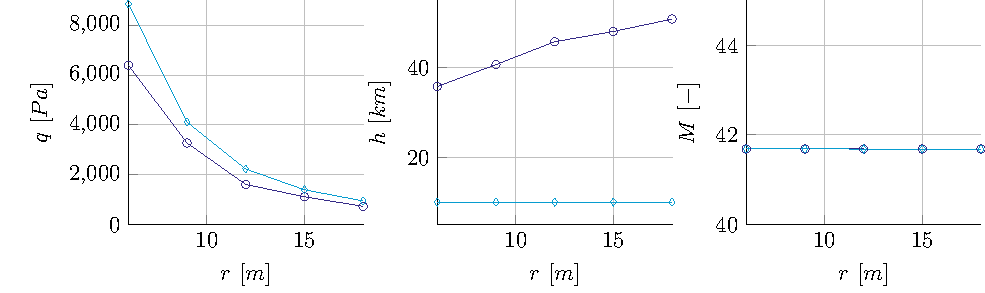
\includegraphics[width=1\textwidth]{./Figure/orbit/radius_param.pdf}
	\caption{maximal dynamic pressure, height and Mach number for different radii}
	\label{fig:radius}
\end{figure}

\paragraph{Entry corridor}
The entry corridor is the fictional box where the re-entry vehicle should pass through to go into orbit. To low and the acceleration limit or the heat limit is breached, to high and the re-entry vehicle will skip on the atmosphere and never return. This corridor is dependent on different design parameters, the most important are the aerodynamic coefficients, entry velocity and control system.

\paragraph{Effect of initial flight path angle}

\paragraph{Effect of angle of attack}

\paragraph{Effect of bank angle}



